% Document class and packages
\documentclass[letterpaper, 12pt]{article}
\usepackage[utf8]{inputenc}
\usepackage[T1]{fontenc}
\usepackage{geometry}
\usepackage{titlesec}
\usepackage{enumitem}

\usepackage{amsmath, amssymb,lipsum,fancyhdr,graphicx,listings,xcolor,color}

% Page setup
\geometry{margin=1in}
\pagestyle{fancy}
\fancyhf{}
\rhead{\thepage}
\lhead{\textit{Audio \& Image Compression - Assignment 3 - Image}}  % Escape '&' with '\&'

% Section and list formatting
\titleformat{\section}[block]{\normalfont\Large\bfseries}{\thesection}{1em}{}[]
\setlist[itemize]{left=0pt, label=--, itemsep=4pt}

% Document information
\title{Audio \& Image Compression}
\author{Bashar Beshoti (207370248)
}
\date{\today}

\begin{document}

% First page: Course details and author information
\maketitle

\section*{Course Information}
\begin{itemize}
    \item \textbf{Course Title:} Audio \& Image Compression  % Escape '&' with '\&'
    \item \textbf{Course Code:} 203.3880
    \item \textbf{Assignment :} Final assignment - Image
    \item     \textbf{Due Date : } 04.04.2024

\end{itemize}
\definecolor{dkgreen}{rgb}{0,0.6,0}
\definecolor{gray}{rgb}{0.5,0.5,0.5}
\definecolor{mauve}{rgb}{0.58,0,0.82}

\lstset{frame=tb,
  language=Python,
  aboveskip=3mm,
  belowskip=3mm,
  showstringspaces=false,
  basicstyle={\small\ttfamily},
  numbers=none,
  numberstyle=\tiny\color{gray},
  keywordstyle=\color{blue},
  commentstyle=\color{dkgreen},
  stringstyle=\color{mauve},
  breaklines=true,
  tabsize=3,
  frame=single
}

\newpage

\section{Block Truncation Coding (BTC)  }
\begin{align*}
    \boxed{\hat{x} = \frac{1}{n^2}\sum_{i} x_i , \sigma = \sqrt{(x^2 - \hat{x}^2)}}
\end{align*}
With this method, the average and standard deviation are found for each block:
Transfer (to the receiver) for each pixel '1' or '0' respectively, '1' if it is higher than the average or '0' if it is lower than average.\\
ONLY THE '0' AND '1' MATRIX IS TRANSFERRED TO THE RECEIVER.\\
In reconstruction (at the receiver), in order to preserve the above two statistical moments, each pixel is "reconstructed" according to the formula:
\[x^- = {\hat{x}-\sigma \cdot \sqrt{\frac{n_{above}}{n_{under}}}} , x^+ = {\hat{x}+\sigma \cdot \sqrt{\frac{n_{above}}{n_{under}}}}\]
That is, pixels for which '0' was transferred get an average value minus the standard deviation multiplied by the constant in the root, and those who received a value of '1' receive the average value plus the standard deviation multiplied by a constant inside the root (note that these are inverse constants!).\\

\begin{itemize}
    \item $n_{above}$ - The number of pixels that received a value of '1'
    \item $n_{under}$ - The number of pixels that received a value of '0'
\end{itemize}

\subsection{A block of pixels (0-255) with a size of 4x4 should be produced where the average of the block will be two digits the last of your ID number and the standard deviation will be the mean divided by the third digit from the end.}
If a special problem arises - for example if the dividing digit is 0 can be used in the next book after it, etc. It is of course possible to use the assistance of various AI systems

\paragraph{Answer :}    
My ID is 207370248. Then, the average is 48 and the standard deviation is 24.
and now I'm going to create a matrix 4x4 fulfill the requirements above:\\
\[\text{Block} = \begin{pmatrix}
40 &72 &24 &36 \\
16 &37 &60 &38 \\
22 &144 &42 &44 \\
58 &47 &62 &26 \\
\end{pmatrix}\]



\subsection{Show the generated block, and perform the process of finding a '0' or '1' representation for each pixel}
\paragraph{Answer :}
Upon definition written in question's context. We can define the following function.
\[
f_{(x,y)} = \begin{cases} 
1 &  x \in [0,3],y\in[0,3] , Block(x,y) <= Average \\
0 &  x \in [0,3],y\in[0,3], Block(x,y) > Average\\
\end{cases}
\]
Therefore, 
\[\text{Binary Block} = \begin{pmatrix}
0 &1 &0 &0 \\
0 &0 &1 &0 \\
0 &1 &0 &0 \\
1 &0 &1 &0 \\
\end{pmatrix}\]
But if I'm mistakenly misunderstood the question and required the binary format of each value. Here it is :
\begin{figure}[htbp]
    \centering
    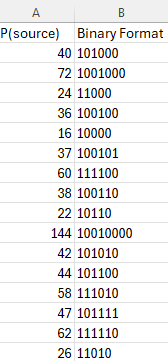
\includegraphics[width=0.25\linewidth]{FINAL_ASSIGNMENT/I_S_3.png}
    \caption{Table of pixels from decimal to binary}
    \label{fig:enter-label}
\end{figure}
\[\text{Binary Format Block} = \begin{pmatrix}
101000 &1001000 &11000 &100100 \\
10000 &100101 &111100 &100110 \\
10110 &10010000 &101010 &101100 \\
111010 &101111 &111110 &11010 \\
\end{pmatrix}_2\]

\subsection{Restore the block based on the process shown above (finding $x^-,x^+$) and perform Quantization by Round to the nearest whole number.}
\paragraph{Answer :}
Based on the Binary Block Matrix, the number of 0's are 11 and number of 1's are 5. So, let's calculate both of $x^+,x^-$ from the equations mentioned above.

\[x^- = {\hat{x}-\sigma \cdot \sqrt{\frac{n_{above}}{n_{under}}}} = {48 +24 \cdot \sqrt{\frac{5}{9}}} \approx 59 \]
\[x^- = {\hat{x} - \sigma \cdot \sqrt{\frac{n_{above}}{n_{under}}}} = {48 -24 \cdot \sqrt{\frac{5}{9}}} \approx 37 \]

\[\text{Quantized Block} = \begin{pmatrix}
37 &59 &37 &37 \\
37 &37 &59 &37 \\
37 &59 &37 &37 \\
59 &37 &59 &37 \\
\end{pmatrix}\]
  
\subsection{The statistical moments for the created block must be calculated - were they really saved?}
\paragraph{Answer :}
if i understand correctly from the response in questions forum i asked, statistical moments is average. so to reshape the question be like:
Calculate the average for the created Block which is : 
\[average' = \frac{1}{n^2}\sum_{0\leq i,j\leq} Quanatized-Block(i,j) = \frac{1}{4^2}\left(11\cdot 39 + 5\cdot 59 \right) = 43.875\]

\subsection{Compute the MSE between the original block and the reconstructed block.}
\paragraph{Answer : }
\begin{figure}[htbp]
    \centering
    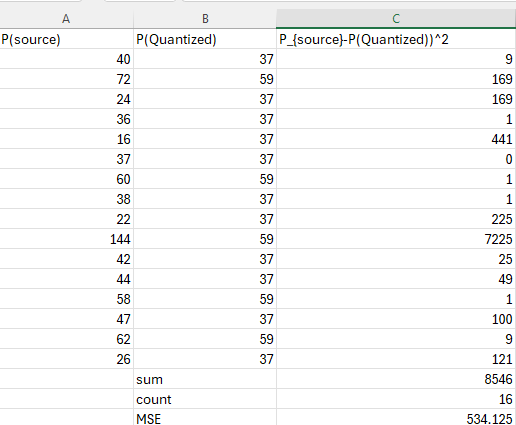
\includegraphics[width=0.75\linewidth]{FINAL_ASSIGNMENT/I_S_5.png}
    \caption{MSE Calculation}
    \label{fig:enter-label}
\end{figure}
\[MSE = \frac{1}{n^2}\sum(P_{source}-P(Quantized))^2 = 534.125\]

\subsection{Calculate the compression ratio between the original block and the compressed block.}
\paragraph{Answer :}
\[Compression-Ratio = \frac{Original-Data-Size}{Compressed-Data-Size}\]
Since each pixel value from Original Block is a value in range $[0,255]$. then it is represented by 8 bits for each value. the total size of original data block is block size times pixel size.
\[Original-Data-Size = (Block-Size) \times (Pixel-Size) = 16 * 8 bits = 144bits \]
\[Compressed-Data-Size = (Block-Size) \times (Pixel-Size) = 16 * 6 bits = 96bits \]

\[Compression-Ratio = \frac{Original-Data-Size}{Compressed-Data-Size} = \frac{144}{96} = \frac{4}{3}\]

\subsection{Infer conclusions quality of compression and recovery for the original block.}
\paragraph{Answer :}
\subparagraph{SNR,PSNR Calculation:}

\begin{table}
    \centering
    \begin{tabular}{|c|c|c|} \hline 
         &  ORIGINAL& COMPRESSED\\ \hline 
         SNR&  1.977336545354818& 1.977336545354818\\ \hline 
         PSNR&  20.854374550426577& 20.854374550426577\\ \hline
    \end{tabular}
    \caption{SNR,PSNR Calculation}
    \label{tab:my_label}
\end{table}

We can infer that :
\begin{enumerate}
    \item Compression Ratio: The compression ratio gives an idea of how much the data has been compressed. A higher compression ratio means more compression, but it may also lead to more loss of information. After achieving a compression ratio of $\frac{4}{3}:1$, meaning the compressed block requires $\frac{4}{3}$ times less data compared to the original block. 
    \item Mean Squared Error (MSE): The MSE between the original block and the reconstructed block gives a measure of the error introduced by the compression and reconstruction process. The MSE in this context equals to 534.125. A lower MSE means less error and better quality of reconstruction.
    \item Signal-to-Noise Ratio (SNR) and Peak Signal-to-Noise Ratio (PSNR): These metrics give a measure of the quality of the reconstructed block compared to the original block. A higher SNR or PSNR means better quality of reconstruction. Based on Table above, we can induce that there the signal power is bigger than the noise especially since both PSNR \& SNR are positive values.
\end{enumerate}


\subsection{Bonus 5 points:}
Claim: There is a certain mathematical relationship between this method and JPEG's method - do you think this claim is true
correctly? You have to reason!
\paragraph{Answer :}
Yes, the claim that there is a certain mathematical relationship between Block Truncation Coding (BTC) and JPEG's method is \textbf{correct}. \\

\subparagraph{Quantization}

Both BTC and JPEG rely on a fundamental mathematical concept called \textit{Quantization} to achieve image compression. This process aims to reduce the number of bits needed to represent the image data by discarding or scaling down certain information.

 BTC performs a simpler form of quantization during image restoration. It uses the average $(\hat{x})$ and standard deviation $(\sigma)$ of each block to restore pixel values.
 JPEG employs a more sophisticated form of quantization based on the Discrete Cosine Transform (DCT) as we learned in lectures. This transform converts the image data from the spatial domain (pixel intensity values) to the frequency domain.  

\begin{figure}[htbp]
    \centering
    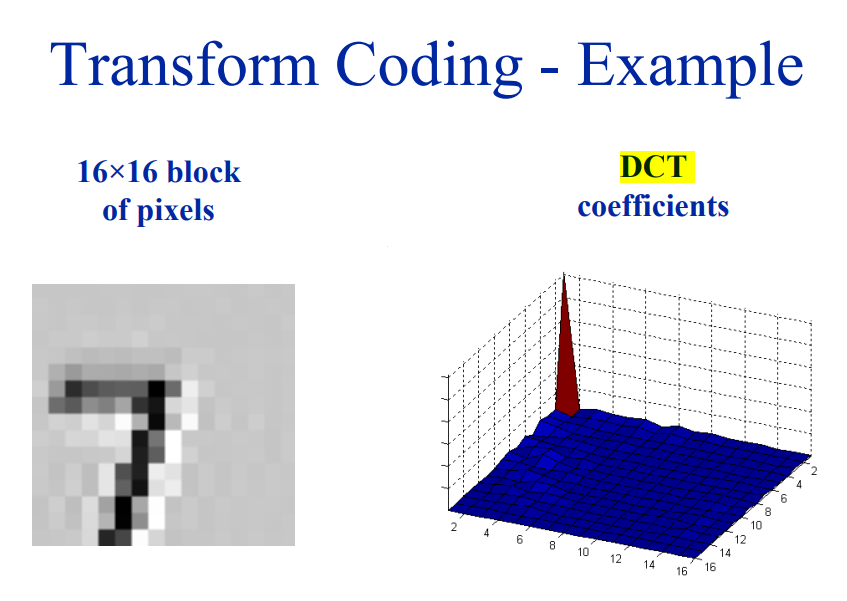
\includegraphics[width=0.75\linewidth]{FINAL_ASSIGNMENT/Example.png}
    
    
\end{figure}
 \textbf{Differences:}
\begin{itemize}
    \item Time Complexity: BTC's quantization is simpler and less computationally expensive compared to JPEG's DCT-based approach.
    \item Concept : BTC quantizes based on average, standard deviation, and category proportions. JPEG targets specific frequencies based on human visual perception for better compression efficiency.
\end{itemize}

 \textbf{Similarities:}
\begin{itemize}
    \item Reducing the number of bits needed to represent the image data.
    \item Introducing controlled information loss for compression.
\end{itemize}
 











\newpage
\section{Code}
\subsection*{Implementation:}
\begin{lstlisting}
import numpy as np

original_block = np.array([[40, 72, 24, 36],
                           [16, 37, 60, 38],
                           [22, 144, 42, 44],
                           [58, 47, 62, 26]])

signal_power = np.var(original_block)

reconstructed_block = np.ones(original_block.shape) * 37
reconstructed_block[original_block > 48] = 59  # Replace elements less than or equal to average with 59

MSE = np.sum(original_block - reconstructed_block) ** 2

noise_power = np.mean((original_block - reconstructed_block) ** 2) # => 534.125
# noise_power = np.var(original_block - reconstructed_block) => 517.109375

snr = 10 * np.log10(signal_power / noise_power)

max_pixel_value = 255  # Assuming 8-bit grayscale image
psnr = 10 * np.log10(max_pixel_value**2 / noise_power)

print('Original matrix:')
print(original_block)

print('reconstructed_block matrix:')
print(reconstructed_block)

print('diff mat')
print(np.abs(original_block - reconstructed_block))


print('MSE IS = ' + str(MSE))


print('noise_power IS = ' + str(noise_power))

print('snr IS = ' + str(snr))

print('psnr IS = ' + str(psnr))
\end{lstlisting}


\subsection*{Output}

\begin{lstlisting}
Original matrix:
[[ 40  72  24  36]
 [ 16  37  60  38]
 [ 22 144  42  44]
 [ 58  47  62  26]]
reconstructed_block matrix:
[[37. 59. 37. 37.]
 [37. 37. 59. 37.]
 [37. 59. 37. 37.]
 [59. 37. 59. 37.]]
diff mat
[[ 3. 13. 13.  1.]
 [21.  0.  1.  1.]
 [15. 85.  5.  7.]
 [ 1. 10.  3. 11.]]
MSE IS = 4356.0
noise_power IS = 534.125
snr IS = 1.977336545354818
psnr IS = 20.854374550426577

=== Code Execution Successful ===
\end{lstlisting}



\end{document}